\documentclass{article}
\usepackage{listings}
\usepackage{xcolor}
\usepackage[margin=1in]{geometry}
\usepackage{amsmath,amsthm,amssymb}
\usepackage{graphicx}
\usepackage{epstopdf}
\DeclareGraphicsExtensions{.eps,.ps,.jpg,.bmp}
\lstset{
	numbers=left,
    framexleftmargin=10mm,
    frame=none,
    backgroundcolor=\color[RGB]{245,245,244},
	keywordstyle=\bf\color{blue},
	identifierstyle=\bf,
	numberstyle=\color[RGB]{0,192,192},
	commentstyle=\it\color[RGB]{0,96,96},
	stringstyle=\rmfamily\slshape\color[RGB]{128,0,0},
	showstringspaces=false
    }

\newcommand{\N}{\mathbb{N}}
\newcommand{\R}{\mathbb{R}}
\newcommand{\Z}{\mathbb{Z}}
\newcommand{\Q}{\mathbb{Q}}

\newenvironment{theorem}[2][Theorem]{\begin{trivlist}
\item[\hskip \labelsep {\bfseries #1}\hskip \labelsep {\bfseries #2.}]}{\end{trivlist}}
\newenvironment{lemma}[2][Lemma]{\begin{trivlist}
\item[\hskip \labelsep {\bfseries #1}\hskip \labelsep {\bfseries #2.}]}{\end{trivlist}}
\newenvironment{exercise}[2][Exercise]{\begin{trivlist}
\item[\hskip \labelsep {\bfseries #1}\hskip \labelsep {\bfseries #2.}]}{\end{trivlist}}
\newenvironment{problem}[2][Problem]{\begin{trivlist}
\item[\hskip \labelsep {\bfseries #1}\hskip \labelsep {\bfseries #2.}]}{\end{trivlist}}
\newenvironment{question}[2][Question]{\begin{trivlist}
\item[\hskip \labelsep {\bfseries #1}\hskip \labelsep {\bfseries #2.}]}{\end{trivlist}}
\newenvironment{corollary}[2][Corollary]{\begin{trivlist}
\item[\hskip \labelsep {\bfseries #1}\hskip \labelsep {\bfseries #2.}]}{\end{trivlist}}

\begin{document}

\title{Homework 2016-03-18}
\author{Chuan Lu\\
13300180056}

\maketitle

\begin{problem}{1}
\text{ }\\
Analysis the stability and absolute stable interval of Modified and Revised Euler Iteration for Dahlquist test.
\end{problem}

\begin{proof}
\subsection{For Modified Euler Iteration:} 
{\centering \[\ u_{n+1} = u_{n} + \frac{\Delta t}{2}(f_{n} + f_{n+1})\]}
\quad Assume that the disturbed initiate value is $\widetilde{u_{0}}$ and the exact initiate value is $u_{0}$. Mark the following value calculated by the Modified Euler Iteration as $\widetilde{u_{i}}, i = 1, 2, \cdots$. Then $\widetilde{u_{n}} = \widetilde{u_{n-1}} + \frac{\Delta t}{2}(a\widetilde{u_{n-1}} + a\widetilde{u_{n}}), \quad \widetilde{u_{n}} = \frac{1+\frac{a\Delta t}{2}}{1 - \frac{a\Delta t}{2}}\widetilde{u_{n-1}},\quad u_{n} = \frac{1+\frac{a\Delta t}{2}}{1 - \frac{a\Delta t}{2}}u_{n-1}$.\quad Hence, $\Vert\widetilde{u_{n}} - u_{n}\Vert =  \frac{1+\frac{a\Delta t}{2}}{1 - \frac{a\Delta t}{2}}\Vert\widetilde{u_{n-1}} - u_{n-1}\Vert = \dots = (\frac{1+\frac{a\Delta t}{2}}{1 - \frac{a\Delta t}{2}})^{n}\Vert\widetilde{u_{0}} - u_{0}\Vert.$\\
\quad If we expect that to a fixed $\Delta t$, when $n\to\infty$, the error can still be of control, then it must be true: $$\Arrowvert\frac{1+\frac{a\Delta t}{2}}{1 - \frac{a\Delta t}{2}}\Arrowvert\leqslant 1.$$ Hence, because that $\Delta t \geqslant 0,$ it can only be true when $a\leqslant 0,$ and $0\leqslant\Delta t < \frac{2}{\vert a\vert}.$\\
\quad On the other hand, take $z = a\Delta t,$ we have $\Arrowvert\frac{2+z}{2-z}\Arrowvert\leqslant 1, \quad z\in\mathcal{Z}.$

\subsection{For Revised Euler Iteration:}
{\centering \[\ u_{n+1} = u_{n} + \Delta ta(u_{n} + \frac{\Delta t}{2}au_{n})\]}
\quad Claimed as above, we have $\widetilde{u_{n+1}} = \widetilde{u_{n}}(1+\Delta ta + \frac{1}{2}(\Delta ta)^{2}).$ Hence, $\Vert\widetilde{u_{n}} - u_{n}\Vert = (1+\Delta ta + \frac{1}{2}(\Delta ta)^{2})^{n}\Vert\widetilde{u_{0}} - u_{0}\Vert.$ As shown above, $\Vert 1+\Delta ta+\frac{1}{2}(\Delta ta)^{2}\Vert\leqslant 1.$
\quad On the other hand, take $z = a\Delta t, $ we have $\Vert z^{2} + 2z + 2\Vert\leqslant 2.$
\end{proof}


% \begin{proof}
% \subsection{The code is shown as follows.}
% \begin{lstlisting}[language={MATLAB}]
% function [ point, weight ] = gauss_coefficient_legendre( order )
% % Calculate the coefficients of gauss integral formula with legendre
% % polynomial.

% b = 0.5 ./ sqrt(1 - (2 * (1:order)) .^ (-2));
% [v, lambda] = eig(diag(b, 1) + diag(b, -1));
% [point, i] = sort(diag(lambda));
% weight = 2 * v(1, i) .^ 2;

% end
% \end{lstlisting}

% \begin{lstlisting}[language={MATLAB}]
% function [ value ] = gauss_integral( func, order )
% % GAUSS_INTEGRAL Calculate the intergral of func in [0, 1] with
% % Gauss-Legendre Formula.
% if order == 1
%     value = feval(func, 0.5);
%     return
% end
% [point, weight] = gauss_coefficient_legendre(order - 1);
% transfered_point = point * 0.5 + 0.5;
% value = weight * feval(func, transfered_point) * 0.5;

% end
% \end{lstlisting}

% \begin{lstlisting}[language = {MATLAB}]
% % get function
% function func = get_func( n )
%     func = @(x)(x .^ n);
% \end{lstlisting}

% \begin{lstlisting}[language = {MATLAB}]
% % homework 4
% clear all;
% result_matrix = zeros(7, 6);
% for n = 1:7
%     func = get_func(n);
%     result_matrix(n, 1) = integral(func, 0, 1);
%     for order = 1:5
%         func = get_func(n);
%         result_matrix(n, order + 1) = gauss_integral(func, order);
%     end
% end
% nlist = 1:5;
% figure(1);
% for i = 1 : 7
%     plot(nlist, result_matrix(i, 2:6) - result_matrix(i, 1));
%     hold on
% end
% title('The error of Gauss-Legendre formula');
% legend('x^1', 'x^2', 'x^3', 'x^4', 'x^5', 'x^6', 'x^7', 'Location', 'Best');
% \end{lstlisting}

% \subsection{The result is shown as follows.}
% \begin{figure}[htbp]
% \centering
% \includegraphics[width = 15cm]{pic1.eps}
% \caption{The relationship of error with order}
% \label{Error}
% \end{figure}
% \end{proof}

\begin{problem}{2}
\text{ }\\
Prove that Implicit Euler Iteration is of first-order convergence for Dahlquist test.
\end{problem}
\begin{proof}
\quad According to (2.2.20), $u_{n} = \frac{1}{(1-a\Delta t)^{n}}u_{0}.$ For $e_{n} = u(t_{n}) - u_{n},$ we have $e_{n} = u_{0}(e^{at_{n}} - e^{-nln(1-a\Delta t)}).$ From Taylor expansion we can know that $$e_{n} = -u_{0}e^{at_{n}}(\frac{a^{2}t_{n}}{2}\Delta t + O(\Delta t^{2})).$$\\
\quad In consequence, for a fixed $T = N\Delta t,$ $\Vert u(T) - u(N)\Vert\leqslant C\Delta t,$ which means the implicit iteration is of first-order convergence.
\end{proof}

\begin{problem}{3}
\text{ } \\
Calculate $\frac{du}{dt} = au$ with Euler Iterations, and show the convergence by pics.
\end{problem}
\begin{proof}
\subsection{The code is shown as follows.}
\begin{lstlisting}[language = {MATLAB}]
function [ t, u ] = Euler_iter( func, inteval, u0, delta_t, op )
% EULER_ITER The main function of Euler Iteration of solving ODEs
% The equation behave likes du/dt = f(t, u), with initial condition given 
% as u(0) = u0 in the inteval [a, b];

% input:
% func : a function of two variables t, u;
% inteval : a list of the inteval of the equation, given like [a, b];
% u0 : the initial condition;
% delta_t : the step size of time;
% op : the kind of iterations, chosen from "explicit', 'implicit',
% 'modified', 'revised';

% output:
% t : the list of time, inited by the inteval and delta_t;
% u : the value of u at the points in t;

if nargin < 2
    error('More arguments needed --Euler-iter');
elseif nargin == 2
    u0 = 1;
    delta_t = 1/8;
    op = 'explicit';
elseif nargin == 3
    delta_t = 1/8;
    op = 'explicit';
elseif nargin == 4
    op = 'explicit';
end

if length(inteval) ~= 2 || inteval(1) >= inteval(2)
    error('Invalid inteval --Euler-iter');
end

switch op
    case 'explicit'
        [t, u] = explicit_iter(func, inteval, u0, delta_t);
    case 'implicit'
        [t, u] = implicit_iter(func, inteval, u0, delta_t);
    case 'modified'
        [t, u] = modified_iter(func, inteval, u0, delta_t);
    case 'revised'
        [t, u] = revised_iter(func, inteval, u0, delta_t);
    otherwise
        error('Invalid operation --Euler-iter');
end

end
\end{lstlisting}

\begin{lstlisting}[language = {MATLAB}]
function [ t, u ] = explicit_iter( func, inteval, u1, delta_t )
% EXPLICIT_ITER Explicit Euler Iteration

t = inteval(1):delta_t:inteval(2);
n = length(t);
u = zeros(1, n);

for i = 1 : n
    u(i) = u1;
    u1 = u1 + delta_t * feval(func, t(i), u(i));
end
\end{lstlisting}

\begin{lstlisting}[language = {MATLAB}]
function [t, u] = implicit_iter(func, inteval, u1, delta_t)
% IMPLICIT_ITER Implicit Euler Iteration

t = inteval(1):delta_t:inteval(2);
n = length(t);
u = zeros(1, n);
f = @(u, u0, t, delta_t)(u - delta_t * feval(func, t, u) - u0);

for i = 1 : n - 1
    u(i) = u1;
    t_i = t(i + 1);
    u0 = u1;
    u1 = fsolve(@(u) f(u, u0, t_i, delta_t), 1);
end
u(n) = u1;

end
\end{lstlisting}

\begin{lstlisting}[language = {MATLAB}]
function [t, u] = modified_iter(func, inteval, u1, delta_t)
% MODIFIED_ITER Modified Euler Iteration

t = inteval(1):delta_t:inteval(2);
n = length(t);
u = zeros(1, n);
f = @(u, u0, t, delta_t)(u - delta_t * feval(func, t, u) - u0);

for i = 1 : n - 1
    u(i) = u1;
    t_i = t(i + 1);
    u0 = u1;
    u1 = fsolve(@(u) f(u, u0, t_i, delta_t), 1);
    u1 = u0 + delta_t/2 * (feval(func, t(i), u0) + ...
        feval(func, t_i, u1));
end
u(n) = u1;

end
\end{lstlisting}

\begin{lstlisting}[language = {MATLAB}]
function [t, u] = revised_iter(func, inteval, u1, delta_t)
% REVISED_ITER Revised Euler Iteration

t = inteval(1):delta_t:inteval(2);
n = length(t);
u = zeros(1, n);

for i = 1 : n - 1
    u(i) = u1;
    u_half = delta_t * feval(func, t(i), u(i)) / 2 + u1;
    t_half = (t(i) + t(i + 1))/2;
    u1 = u1 + delta_t * feval(func, t_half, u_half);
end
u(n) = u1;

end
\end{lstlisting}

\begin{lstlisting}[language = {MATLAB}]
% Homework 4-3
clear all;
format long;
a = -2;
func = @(t, u)(a .* u);
u0 = 1;
u1 = -1;
delta_t = 1/8;
inteval = [0, 3];
op = {'explicit', 'implicit', 'modified', 'revised'};
symbol = {'*-', '.-', 'd-', 'o-'};

figure(1);
for i = 1:4
    [t, u] = Euler_iter(func, inteval, u0, delta_t, char(op(i)));
    [t2, u2] = Euler_iter(func, inteval, u1, delta_t, char(op(i)));
    plot(t, u, cell2mat(symbol(i)));
    hold on;
    plot(t2, u2, cell2mat(symbol(i)));
    hold on;
end

exact_func = @(x, u0)(exp(a .* x + log(u0)));
exact_value1 = feval(exact_func, t, u0);
exact_value2 = feval(exact_func, t, u1);
plot(t, exact_value1, 'x-');
hold on;
plot(t, exact_value2, 'x-');
legend('Explicit1', 'Explicit2', 'Implicit1', 'Implicit2',...
    'Modified1', 'Modified2', 'Revised1', 'Revised2',...
    'Exact1', 'Exact2', 'Location', 'Best');
title('Solving ODE du/dt = a*u with Euler Iteration');
grid on;

figure(2);
m = 5;
error_list = zeros(4, m);
for j = 1:m
    delta_t = 2 ^ (-j - 2);
    t = inteval(1):delta_t:inteval(2);
    exact_value = feval(exact_func, t, u0);
    for i = 1:4
        [t, u] = Euler_iter(func, inteval, u0, delta_t, char(op(i)));
        error_list(i, j) = max(abs(u - exact_value));
    end
end
for i = 1 : 4
    loglog(2 .^ (-3:-1:-m-2), error_list(i, :), cell2mat(symbol(i)));
    hold on;
end
legend('Explicit', 'Implicit', ...
    'Modified', 'Revised', ...
    'Location', 'Best');
title('Error of Euler iterations of solving du/dt = a*u');
grid on;
\end{lstlisting}

\subsection{The result is shown as follows.}
\begin{figure}[htbp]
\centering
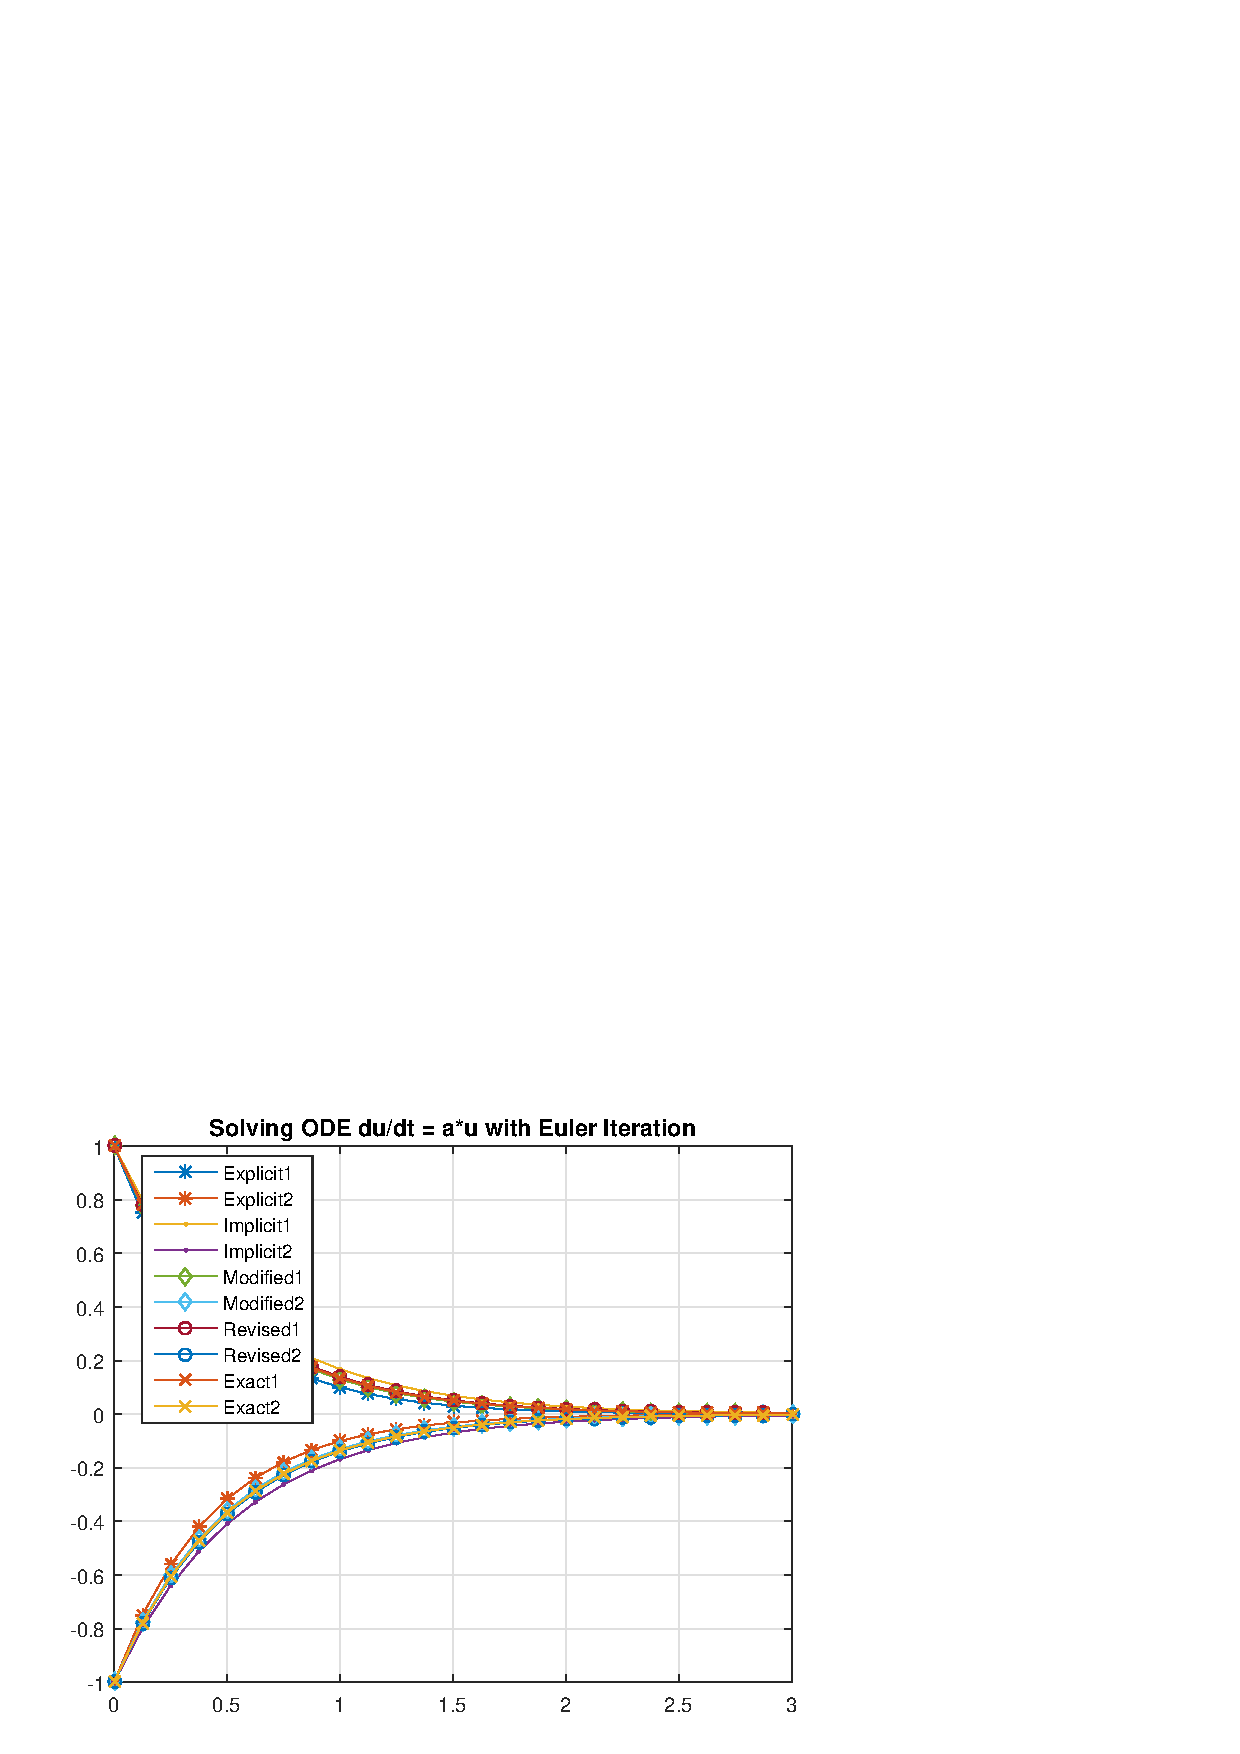
\includegraphics[width = 15cm]{converge.jpg}
\caption{The convergence of Euler Iteration.}
\label{Convergence}
\end{figure}
\begin{figure}[htbp]
\centering
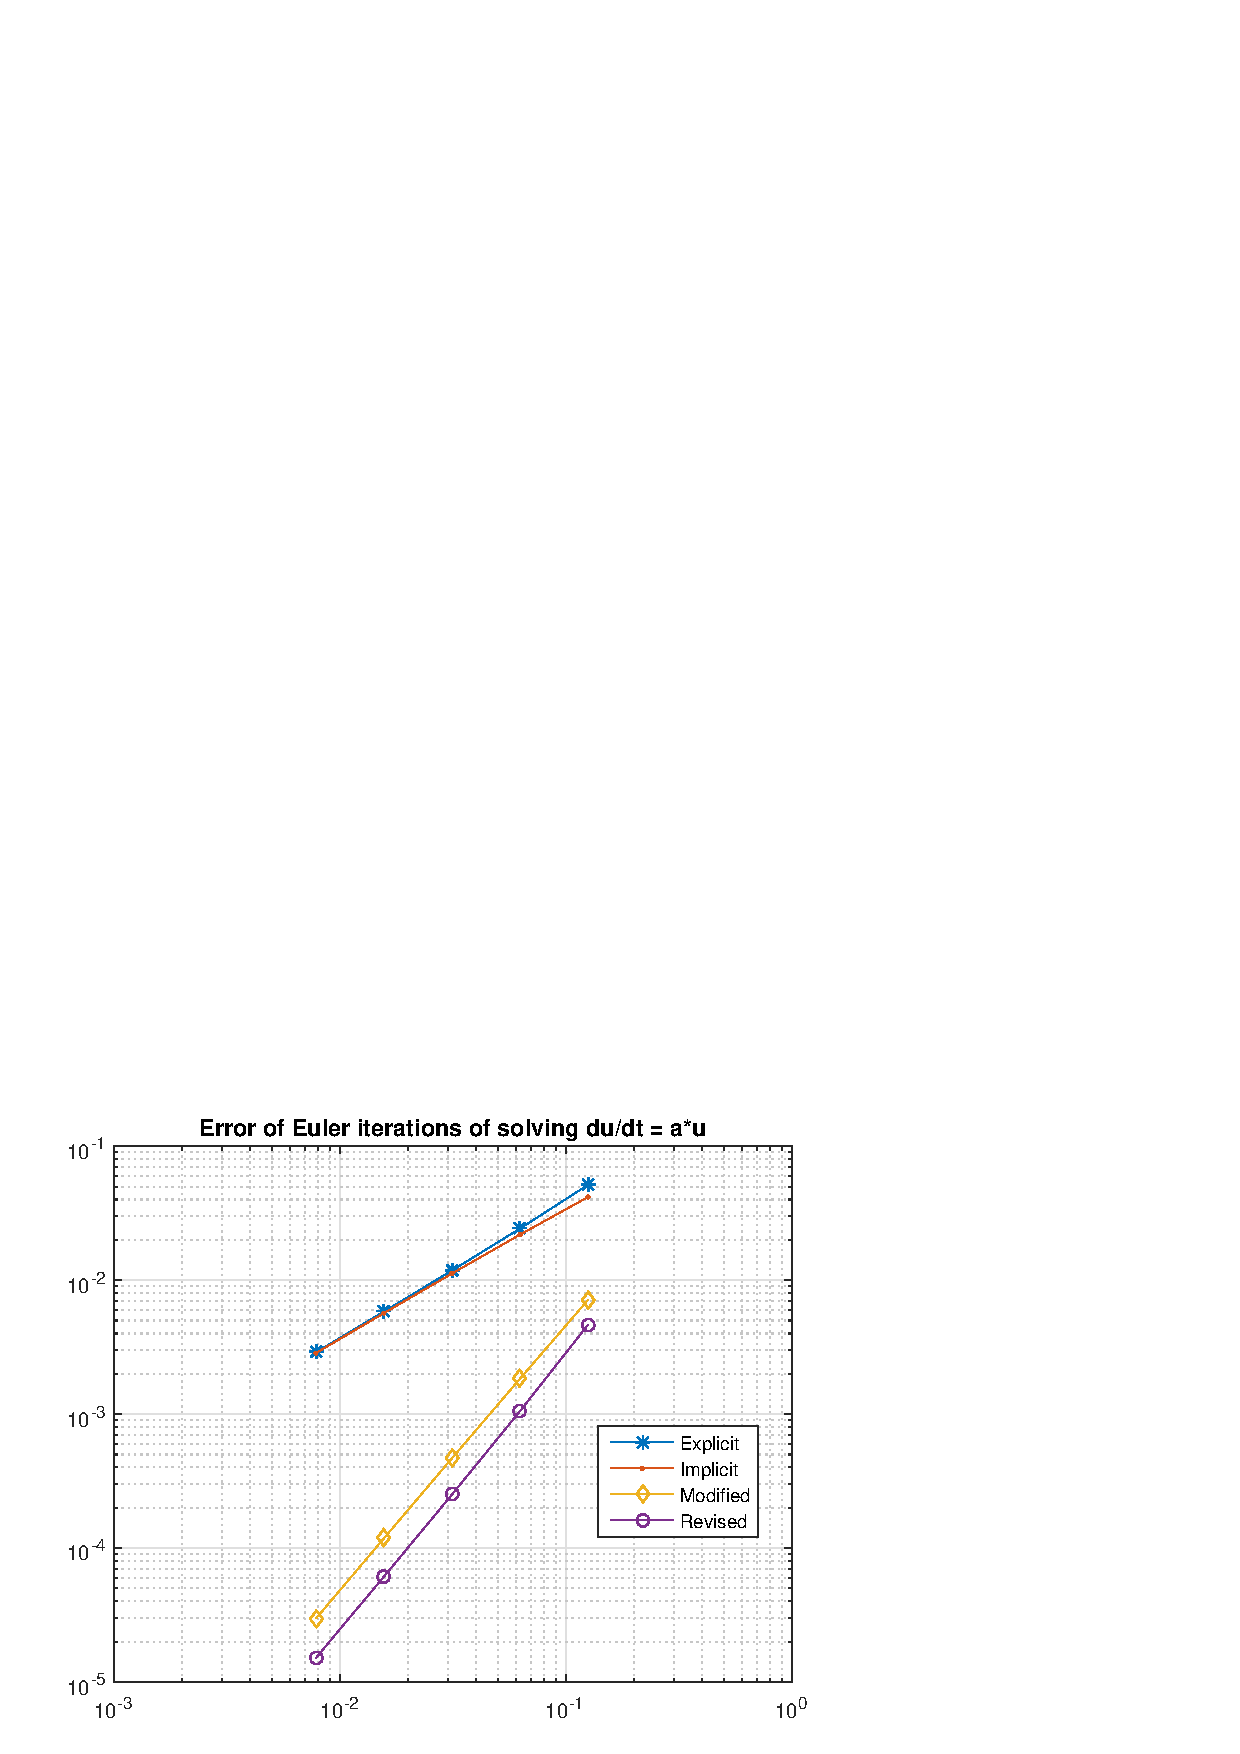
\includegraphics[width = 15cm]{error_list.jpg}
\caption{The error of Euler Iteration.}
\label{Error}
\end{figure}
\end{proof}


% \begin{table}
% \begin{tabular}{c|c|c|c|c|c|c}
%     \hline
%     & Exact Value & medium formula & trapezium formula & Simpson formula & 3/8 formula & Cotes formula \\
%     \hline
%     $x^{1}$ & 0.5000 & 0.5000 & 0.5000 & 0.5000 & 0.5000 & 0.5000 \\
%     \hline
%     $x^{2}$   & 0.3333  &  0.2500  &  0.5000 &  0.3333  &  0.3333  &  0.3333 \\
%     \hline
%     $x^{3}$ & 0.2500  &  0.1250 &   0.5000 & 0.2500  &  0.2500    &    0.2500 \\
%     \hline
%     $x^{4}$  & 0.2000 &   0.0625  &  0.5000  & 0.2083 &   0.2037    &   0.2000 \\
%     \hline
%     $x^{5}$   &  0.1667  &  0.0313 &  1 0.5000 &   0.1875 &  0.1759  &  0.1667 \\
%     \hline
%     $x^{6}$  &   0.1429  &  0.0156  &  0.5000  &  0.1771  &  0.1584  &  0.1432 \\
%     \hline
%     $x^{7}$   &  0.1250  &  0.0078  &  0.5000  &  0.1719   & 0.1471  &  0.1263 \\
%     \hline
%     \end{tabular}
%     \caption{Integral of $x^{n}$ using Newton-Cotes Formula}
%     \end{table}
% \end{proof}
% \end{document}
% \begin{lstlisting}[language={MATLAB}]
% % make matrix
% % author: chuanlu
% % 2016-03-02
% function [A] = make_matrix(op, n)

%     if nargin < 1
%         error('More args needed --make matrix');
%     elseif nargin == 1
%         op = 'A1';
%     end

%     if op == 'A1'
%         c1 = zeros(1, n - 1);
%         c1(2 : n - 1) = -3;
%         c2 = zeros(1, n - 2) + 2;
%         A = eye(n) + diag(c1, -1) + diag(c2, -2);
%     elseif op == 'A2'
%         c1 = zeros(1, n - 1);
%         c1(2 : n - 1) = -3;
%         c2 = zeros(1, n - 2) + 2;
%         A = eye(n) + diag(c1, -1) + diag(c2, -2);
%         A(1, n) = -1;
%     else
%         error('Operation Failed to Match A1 or A2');
%     end
% \end{lstlisting}

% \begin{lstlisting}[language={MATLAB}]
% % homework2.m
% % author: chuanlu
% % 2016-03-02

% op1 = 'A1';
% op2 = 'A2';
% N = 100;
% cond1 = zeros(1, N);
% cond2 = zeros(1, N);
% for n = 1 : N
%     A1 = make_matrix(op1, n);
%     A2 = make_matrix(op2, n);
%     cond1(n) = cond(A1);
%     cond2(n) = cond(A2);
% end
% n = [1:N];
% figure(1);
% semilogy(n, cond1, '*-');
% figure(2);
% plot(n, cond2, '*-');
% %     disp('cond1:');
% %     disp(cond1);
% %     disp('cond2:');
% %     disp(cond2);
% \end{lstlisting}
% The result is shown as follows.
% \end{proof}

% \begin{problem}{3}
% \text{ }\\
% Given $\Vert x_{n+2} - x_{n+1} \Vert$  $\leqslant$ $\alpha\Vert x_{n+1} - x_{n} \Vert$, then $\Vert x^{\star} - x_{n} \Vert$ $\leqslant$ $\frac{\alpha_{n}}{1-\alpha}\Vert x_{1} - x_{0}\Vert$.
% \end{problem}

% \begin{proof}
% $\Vert x_{n} - x_{n - 1} \Vert\leqslant\alpha\Vert x_{n - 1} - x_{n - 2} \Vert\leqslant\dots\leqslant\alpha^{n-1}\Vert x_{1} - x_{0}\Vert$ \\
% \par Hence, $\Vert x_{\star} - x_{n} \Vert\leqslant\Vert x_{n} - x_{n+1} \Vert+\Vert x_{n+1} - x_{n+2}\Vert + \dots\leqslant(\alpha^{n}+\alpha^{n+1}+\dots)\Vert x_{1} - x_{0}\Vert$ \\
% \par$= \frac{\alpha^{n}}{1-\alpha}\Vert x_{1} - x_{0}\Vert$

\end{document}
% % \begin{problem}{4}
% % \text{ }\\
% % Suppose that $[a]$ is a unit in $\Z_{n}$ and $[b]$ is an element of $\Z_{n}$. Prove that the equation $[a]x = b$ has exactly one solution in $\Z_{n}$
% % \end{problem}

% % \begin{proof}

% % \end{proof}

% % \begin{problem}{5}
% % \text{ }\\
% % Suppose that $[a]$ and $[b]$ are both units in $\Z_{n}$.  Show that the product $[a] \cdot [b]$ is also a unit in $\Z_{n}.$ (Note that this confirms closure under multiplication in the group $U_{n})$.
% % \end{problem}

% % \begin{proof}

% % \end{proof}

% % \begin{problem}{6}
% % \text{ }\\
% % Which of the following are Groups? Which of the following are not groups, and why?\\

% % \indent (1)  $G = \{{2, 4, 6, 8}\}$ in $\Z_{10}$.  Where $a \star b = ab$\\
% % \indent (2)  $G = \Q^{\ast}$, where $a \star b = \frac{a}{b}$\\
% % \indent (3) $G = \Z$, where $a \star b = a - b$\\
% % \indent (4) $G = \{ {2^{x}\mid x \in \Q} \}$, where $a \star b = ab$\\

% % \end{problem}

% % \begin{proof}

% % \end{proof}

% % \begin{problem}{7}
% % \text{ }\\
% % Consider the set $Q =$ \{ $\pm$1, $\pm$i, $\pm$j, $\pm$k\} of the complex matrices as follows:\\
% % \[
% % 1=
% %   \begin{bmatrix}
% %     1 & 0\\
% %     0 & 1\\
% %   \end{bmatrix}
% % \]

% % \[
% % i=
% %   \begin{bmatrix}
% %     i & 0\\
% %     0 & $-$i\\
% %   \end{bmatrix}
% % \]

% % \[
% % j=
% %   \begin{bmatrix}
% %     0 & 1\\
% %     $-$1 & 0\\
% %   \end{bmatrix}
% % \]

% % \[
% % k=
% %   \begin{bmatrix}
% %     0 & i\\
% %     i & 0\\
% %   \end{bmatrix}
% % \]
% % Show that $Q$ is a group under matrix multiplication by writing out its multiplicaiton table. (Note: $Q$ is called the quartenion group).
% % \end{problem}
% % \begin{proof}

% % \end{proof}

\end{document}
